\documentclass{template}
\usepackage{float}
\usepackage{mathtools}
\usepackage{listings}
\usepackage{color}

\definecolor{dkgreen}{rgb}{0,0.6,0}
\definecolor{gray}{rgb}{0.5,0.5,0.5}
\definecolor{mauve}{rgb}{0.58,0,0.82}

\lstset{frame=tb,
  aboveskip=3mm,
  belowskip=3mm,
  showstringspaces=false,
  columns=flexible,
  basicstyle={\small\ttfamily},
  numbers=none,
  breaklines=true,
  breakatwhitespace=true,
  tabsize=3
}
\DeclarePairedDelimiter{\simset}{\{}{\}}
\titolo{Fuji Sushi}
\descrizione{Relazione del progetto di Tecnologie Web.}
\versione{1.0} 
\data{2022-06-02}
\responsabile{Giacomo Stevanato}
\redattori{Daniele Trentin}
\verificatori{Christian Micheletti}
\stato{Approvato}
\destinatari{DeltaX \\ Prof. Riccardo Cardin \\ Prof. Tullio Vardanega}
\uso{Interno}

\begin{document}
\firstpage
\tableofcontents
\pagebreak

	\begin{center}
		\textbf{\large Informazioni sul sito} \\
		Indirizzo del sito web \href{http://tecweb.studenti.math.unipd.it/srizzato/}{http://tecweb.studenti.math.unipd.it/srizzato/}\\
		Referente del gruppo: Samuele Rizzato 1226307 \\
		Mail del referente: samuele.rizzato.1@studenti.unipd.it\\
		Email MyWcag4All: luciano.wu@studenti.unipd.it\\
		Account MyWcag4All: luciano
	\end{center}
	
	\begin{table}[H]
		\centering
		\begin{tabular}{|l|l|l|}
			\hline
			\textbf{Tipologia di utente}	& \textbf{Username}	& \textbf{Password} \\
			\hline
			Amministratore	        		& admin				& admin \\
			\hline
			Utente generico					& user				& user \\
			\hline
		\end{tabular}
		\caption{Credenziali degli utenti del sito.}
	\end{table}

\pagebreak

	\section{Introduzione}
	\subsection{Abstract}
    \textit{Fuji Sushi} è un piccolo ristorante dai sapori orientali che sta rapidamente conquistando il mercato, al fine di consolidare e mantenere questa scia di successo il ristorante ha deciso di rinnovare il proprio sito \textit{web} per l'acquisto e recapito dei loro deliziosi piatti. \\
    Il nuovo sito vuole essere un passo avanti alla concorrenza, la quale solitamente espone solo un catalogo statico del loro menù, perciò Fuji Sushi mette a disposizione un vasto repertorio di funzionalità per tutti i suoi utenti.
    La funzionalità cardine riguarda la visualizzazione e l'acquisto dei piatti offerti dal ristorante, ma il sito offre anche molte altre comodità, tra cui:
    \begin{itemize}
        \item un sistema di filtraggio per il vasto menù;
        \item un \textit{feed} delle ultime notizie del ristorante. per rimanere sempre aggiornati sulle ultime novità;
        \item un servizio di \textit{take-away}, con la possibilità di ordinare ad orari flessibili e programmati a discrezione dell'utente;
        \item un carrello intelligente che ricorda le scelte del cliente, anche se non autenticato;
        \item un sistema di notifica per dare un \textit{feedback} all'utente delle sue azioni;
        \item molte altre azioni per gli utenti autenticati.
    \end{itemize}
    Oltre ad essere funzionale il sito vuole anche essere informativo, fornendo una pagina per i contatti rilevanti e una pagina che suggerisce i migliori piatti del momento. \\
    Nonostante il sito ruoti attorno all'utente, l'autenticazione non è obbligatoria: i visitatori hanno comunque il pieno accesso al sito, al menù e anche al carrello, ma ovviamente non sono abilitati all'acquisto. \\
    Infine il sito segue una serie di convenzioni e idee progettuali che si sono rivelate di successo nel tempo, quali:
    \begin{itemize}
        \item rispetto degli standard \textit{W3C}, \textit{HTML5} e \textit{CSS3};
        \item netta separazione tra struttura, presentazione, comportamento;
        \item adesione alle regole di accessibilità, con gli standard \textit{WAI-ARIA} e WCAG (AAA).
    \end{itemize}

	\subsection{Analisi dell'utenza}
    
    \begin{figure}[H]
		\centering
		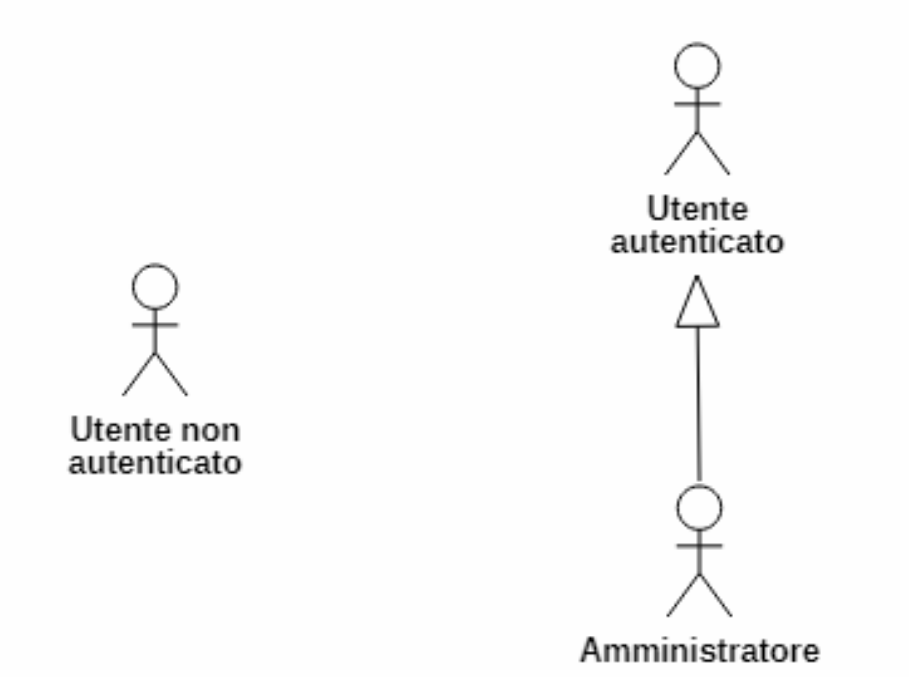
\includegraphics[scale=0.2]{src/gerarchia_utenti.png}
		\caption{Gerarchia degli utenti.}
	\end{figure}

	Il sito web si rivolge prevalentemenete agli amanti del sushi, le funzionalità sono state pensate per favorire i diversi bisogni dell'utente durante l'ordine, ponendo l'attenzione sulla flessibilità degli acquisti, tramite un servizio di recapito o \textit{take-away} e una pianificazione del momento di ritiro. \\
    L'utente generico non autenticato deve poter anche trovare le ultime notizie riguardanti il ristorante, per portarlo a conoscenza di nuovi piatti o eventi, e visualizzare i piatti del momento tramite un \textit{ranking} dei piatti più richiesti. \\
    Il sito è stato anche pensato per l'uso da parte dei gestori, attraverso un sistema di gestione del menù per l'aggiunta o rimozione di piatti e categorie. \\
    L'utenza è così suddivisa:
	\begin{itemize}
		\item \textbf{Utente non autenticato}: ricerca informazioni, visita il menù e le \textit{news}, può aggiungere piatti al carrello ma non può finalizzare gli ordini;
		\item \textbf{Utente autenticato}: ha accesso a tutte le funzionalità di un utente non autenticato, inoltre è abilitato all'acquisto dei piatti scelti e alla gestione del suo profilo personale;
		\item \textbf{Amministratore}: ha accesso a tutte le funzionalità di un utente autenticato, inoltre gestisce il menù e le \textit{news} del ristorante.
	\end{itemize}

	Per quanto riguarda il lato tecnologico, il sito è anche pensato per essere fruibile da dispositivi variegati, implementando quattro diverse viste del sito:
	\begin{itemize}
		\item visualizzazione \textit{desktop};
		\item visualizzazione \textit{tablet};
		\item visualizzazione \textit{mobile};
		\item visualizzazione \textit{desktop}.
	\end{itemize}

	\section{Progettazione}
	\subsection{Struttura del sito}
	\begin{figure}[H]
		\centering
		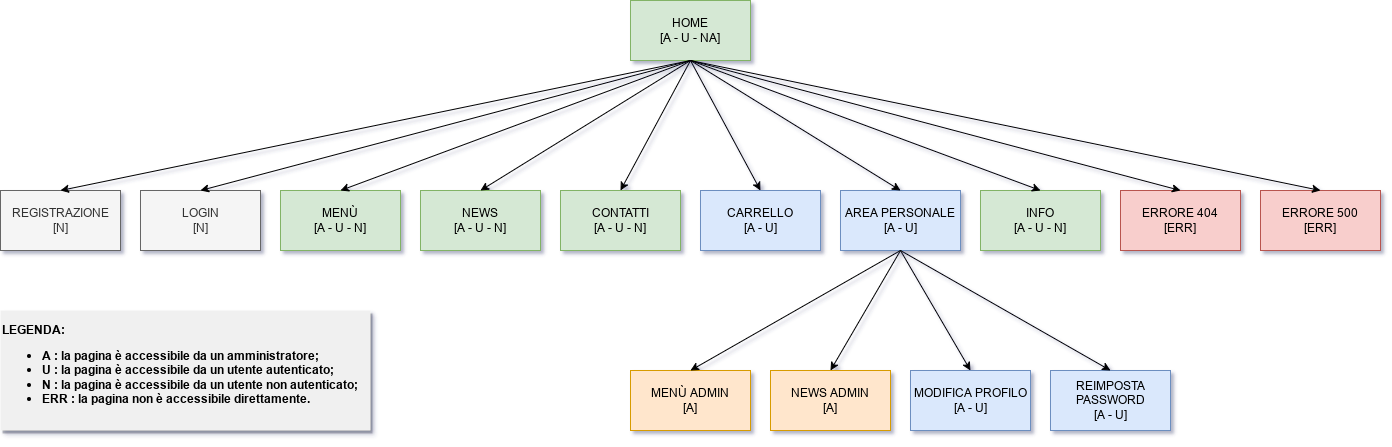
\includegraphics[scale=0.3]{src/mappa_sito.png}
		\caption{Mappa che illustra la struttura del sito.}
	\end{figure}
	
	Il sito è basato su una struttura sia gerarchica che a ipertesto, ogni pagina può accedere ad un'altra pagina sullo stesso livello, tramite degli ipertesti, ma per scendere di livello è necessario passare per la pagina di riferimento. I collegamenti forniti dipendono dai permessi dell'utente, in ciò un utente non autenticato vede quindi una struttura del sito semplificata e di più facile navigazione. \\
	Il sito è stato strutturato seguendo un approccio vicino all'utente, seguendo lo schema a tre pannelli:
	\begin{itemize}
		\item \textbf{Dove sono?}: l'informazione è reperibile nel breadcrumb;
		\item \textbf{Dove posso andare?}: l'informazione è reperibile nella barra superiore di navigazione.
		\item \textbf{Di cosa si tratta?}: l'informazione è reperibile nel titolo della pagina e in quelli delle sezioni;
	\end{itemize} 

	\subsubsection{Header} \label{header}

	\begin{figure}[H]
		\centering
		
\includegraphics[scale=0.3]{src/header.png}
		\caption{Header}
	\end{figure}

	L'\textit{header} è l'elemento di riferimento per la navigazione del sito, è composto di più parti:
	\begin{itemize}
		\item il menù di navigazione a sinistra per spostarsi nelle pagine accessibili da ogni tipologia di utente, visualizzabile in modalità \textit{desktop} e accessibile dal menù a comparsa in modalità \textit{mobile};
		\item il menù di navigazione a destra per spostarsi nelle pagine accessibili dagli utenti autenticati o per eseguire l'accesso, visualizzabile in modalità \textit{desktop} e accessibile dal menù a comparsa in modalità \textit{mobile};
		\item il titolo del sito, composto sia dal logo che dal nome;
		\item il \textit{breadcrumb}, che indica il percorso effettuato per accedere alla pagina in cui ci si trova, fornendo anche i \textit{link} per tornare alle pagine precedentemente visitate;
		\item il \textit{link} per spostare il focus sul contenuto della pagina.
	\end{itemize}
	
	\subsubsection{Contenuto} \label{contenuto}
	Di seguito le pagine che compongono il sito:
	\begin{itemize}
		\item \textbf{\textit{Home}}: è la pagina principale del sito, offre uno sguardo veloce sulle ultime \textit{news} del ristorante e sui piatti del momento, in fondo alla pagina è presente inoltre una breve sezione sulla storia del ristorante e delle funzionalità del sito;
		\item \textbf{Menù}: contiene il catalogo completo dei piatti, divisi per categoria, che l'utente può aggiungere al carrello temporaneo. Il carrello nel menù permette di: salvare il carrello permanentemente, svuotare il carrello, rimuovere dei piatti o modificarne la quantità ordinata; 
		\item \textbf{\textit{News}}: contiene una lista di tutte le notizie del ristorante, dalla più recente alla più vecchia. Ogni \textit{news} è composta di un titolo, un contenuto, una data di pubblicazione e un'immagine rappresentativa;
		\item \textbf{Contatti}: contiene i recapiti, gli orari di lavoro e ulteriori contatti per la comunicazione diretta con il ristorante;
		\item \textbf{Carrello}: visualizza il carrello corrente dell'utente e permette di completare l'ordine;
		\item \textbf{Area personale}: punto di ingresso per la gestione del proprio profilo (per l'utente autenticato) o per la gestione del sito (esclusivo per l'amministratore). L'area personale contiene anche lo storico degli ordini effettuati, visualizzato in formato tabellare;
		\item \textbf{\textit{Login}}: contiene il modulo di autenticazione;
		\item \textbf{Registrazione}: contiene il modulo di registrazione;
		\item \textbf{Menù \textit{admin}}: permette di aggiungere ed eliminare piatti o categorie dal menù;
		\item \textbf{\textit{News admin}}: permette di aggiungere ed eliminare;
		\item \textbf{Modifica profilo}: permette di modificare i dati personali dell'utente;
		\item \textbf{Reimposta \textit{password}}: permette di modificare la password dell'utente;
		\item \textbf{Errore 404}: pagina informativa, indica che la risorsa richiesta non esiste;
		\item \textbf{Errore 500}: pagina informativa, indica che il \textit{server} non è in grado di soddisfare la richiesta;
		\item \textbf{Info}: pagina informativa, indica l'esito di una determinata azione dell'utente.
	\end{itemize}
	
	\subsubsection{Footer}
	All'interno del footer compaiono elementi di generica utilità e informazioni importanti che non sono presenti nel resto del sito:
	\begin{itemize}
		\item i contatti del ristorante;
		\item le tecnologie e gli standard utilizzati per comporre il sito;
		\item gli autori e proprietari del sito.
	\end{itemize}
	
	\subsubsection{Base di dati}

    \paragraph{Schema concettuale}
	\begin{figure}[H]
		\centering
		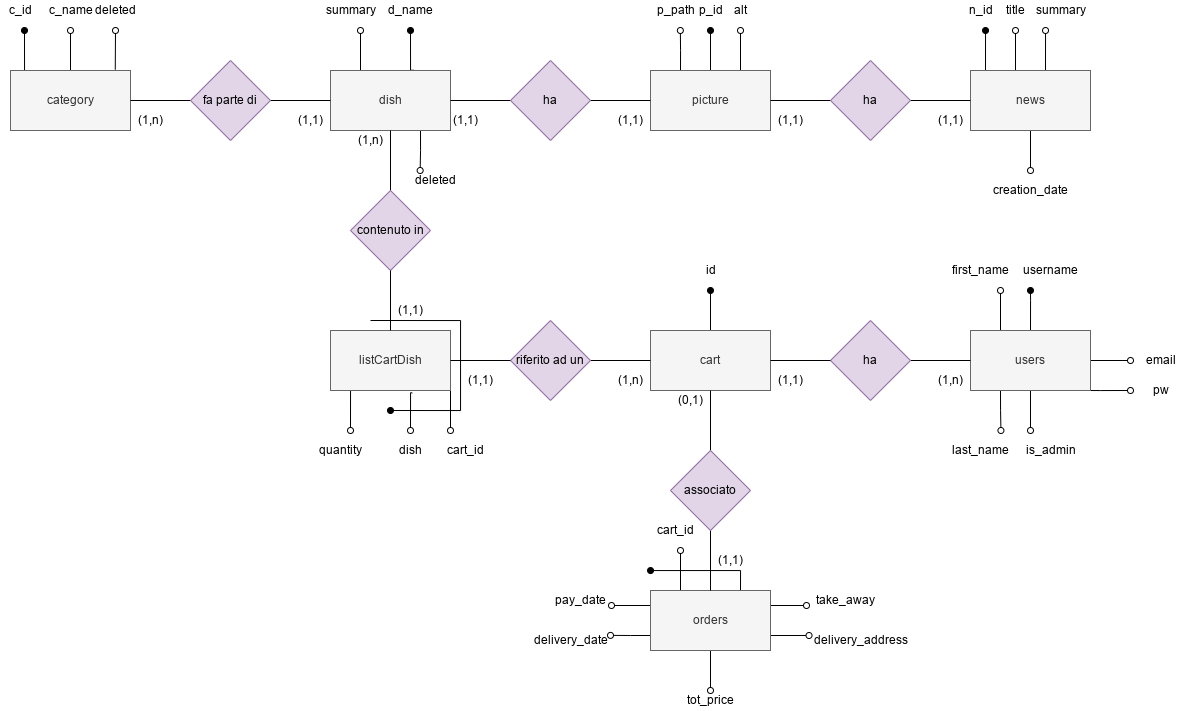
\includegraphics[scale=0.3]{src/db_er.png}
		\caption{Schema concettuale del database.}
	\end{figure}

	La base di dati è stata progettata per supportare le funzionalità offerte dal sito, consentendo di:
	\begin{itemize}
		\item salvare le informazioni di un utente;
		\item contenere i piatti del menù;
		\item inserire ed eliminare nuove categorie;
		\item inserire ed eliminare news;
		\item creare ordini;
		\item mantenere lo stato del carrello.
	\end{itemize}

	La base di dati inoltre è stata scomposta in terza forma normale di Boyce Codd per renderla manutenibile nel tempo.

	\paragraph{Schema logico}
	\begin{lstlisting}
	     category (c_id, c_name, deleted)
        picture (d_name, p_path, alt)
        dish (p_id, summary, price, deleted, category, picture)
        users (username, email, first_name, last_name, pw, is_admin)
        news (n_id, title, summary, creation_date, picture)
        cart (id, users)
        orders (cart_id, pay_date, delivery_date, tot_price, take_away, delivery_address)
        listCartDish (cart_id, dish, quantity)

        dish.category -> category.c_id
        dish.picture -> picture.p_id
        news.picture -> picture.c_id
        cart.users -> users.username
        orders.cart_id -> cart.id
        listCartDish.dish -> dish.d_name
        listCartDish.cart_id -> cart.id
    \end{lstlisting}
    
	\subsubsection{Ricerche probabili}
    Le pagine contengono la seguente lista di parole chiave per facilitare e indirizzare la ricerca dell'utente al nostro sito:
	\begin{itemize}
	\item Fuji;
	\item sushi;
	\item ristorante;
	\item giapponese;
	\item takeaway;
	\item menu;
	\item piatti;
	\item cucina;
	\item pesce.
	\end{itemize}

	\section{Realizzazione}
	\subsection{Linguaggi}
	\begin{itemize}
		\item \textbf{HTML5}: per la struttura del sito, HTML5 offre tag utili per una scrittura semantica delle pagine (header, main, footer...) e molti attributi per controlli \textit{built-in}, come il \textit{pattern} o \textit{required}, e di accessibilità, come gli attributi \textit{ARIA};
		\item \textbf{CSS3}: utilizzato nella parte di presentazione, per costruire un layout \textit{responsive} e fluido, la terza versione offre i nuovi \textit{grid} e \textit{flex} per organizzare il \textit{layout} del menù e struttura le sezioni delle pagine;
		\item \textbf{JavaScript}: per la validazione dei \textit{form} lato \text{client}, per mantenere lo stato locale del carrello dell'utente, per il menù e carrello a comparse. Non è stata utilizzata alcuna libreria esterna e tutte le funzionalità sono state inserite in un unico file per ridurre il tempo di latenza dell'utente;
		\item \textbf{PHP}: utilizzato per gestire la logica di \textit{business} del sito e realizzare pagine \textit{web} dinamiche, per le interazioni col database e la validazione lato \textit{server};
		\item \textbf{SQL}: utilizzato per interagire con la base di dati, tramite \textit{query} per l'inserimento/rimozione/aggiornamento dei dati.
	\end{itemize}


	\subsection{Strumenti}
	\begin{itemize}
		\item \textbf{Google Meet}: per gestire gli incontri del gruppo;
		\item \textbf{GitHub}: per collaborare in modo efficace tra più persone;
		\item \textbf{Server PHP}: per eseguire il sito in locale e testare le sue funzionalità;
		\item \textbf{MySqlWorkbench}: per avere un'interfaccia sullo stato della base di dati;
		\item \href{https://web.math.unipd.it/accessibility-dev/}{\textbf{MyWcag4All}}: per esguire controlli multipli di accessibilità;
		\item \href{https://wave.webaim.org/extension/}{\textbf{Wave Extension}}: per controllare errori strutturali del sito (link mancanti, immagini senza alt...).
		\item \href{https://chrome.google.com/webstore/detail/wcag-color-contrast-check/plnahcmalebffmaghcpcmpaciebdhgdf}{\textbf{WCAG Color Contrast Checker}}: per essere coonformi allo standard WCAG AAA per il contrasto dei colori usati;
		\item \href{https://gsnedders.html5.org/outliner/}{\textbf{HTML outliner}}: per evidenziare errori nella struttura del codice HTML;
		\item \href{https://validator.w3.org/}{\textbf{HTML5 Validator}}: per conformare il codice allo standard HTML5;
		\item \href{https://jigsaw.w3.org/css-validator/}{\textbf{CSS3 Validator}}: per conformare il codice allo standard CSS3.
	\end{itemize}

	\section{Accessibilità}
	Lo standard su cui ci siamo conformati è WCAG 2.0 (\href{https://www.w3.org/Translations/WCAG20-it/}{https://www.w3.org/Translations/WCAG20-it/})

	\subsection{Separazione tra comportamento, struttura e presentazione}
	La separazione tra i diversi aspetti del sito è stata perseguita dividendo in tre parti:
	\begin{itemize}
		\item parte strutturale: con i file \textit{HTML}, definiscono la struttura e le componenti delle pagine in modo statico; 
		\item parte di presentazione: con i file \textit{css}, definiscono l'aspetto delle pagine e delle loro componenti;
		\item parte comportamentale: con i file \textit{javascript}, definiscono le funzioni lato \textit{client} che il sito offre (validazione, carrello locale e menù a comparsa).
	\end{itemize}
	All'interno dei file \textit{HTML} non sono stati integrati tag inerenti alle parti di presentazione o comportamento, gli stili vengono applicati includendo i riferimenti a i file esterni.
	
	\subsection{WAI-ARIA}
	Nel progetto abbiamo deciso di utilizzare lo standard \textit{WAI-ARIA}, più precisamente l'attributo \textit{aria-label} è stato usato al fine di rendere accessibile il \textit{breadcrumb} presente nell'\textit{header} delle pagine.
	Per altri elementi o attributi abbiamo deciso di adottare quelli standard forniti da \textit{HTML}.

	\subsection{Colori}
	Tutti i colori utilizzati superano il test textit{WCAG AAA}, ma non per alcuni tipi di cecità cromatica, dove si raggiunge solo lo standard \textit{AA}, di seguito la \textit{palette} usata;
	\begin{itemize}
		\item \textbf{dark-accent}: \textit{\#1f0707}, è una tinta di rosso scuro tendente al marrone ispirati dalla salsa di soia, usato per gli sfondi delle sezioni e per i bottoni, o per tutto ciò che ha come sfondo un \textit{light-accent};
		\item \textbf{light-accent}: \textit{\#ffffff},è un bianco candido ispirato al riso, usato per lo sfondo del contenuto delle sezioni e per i bottoni inattivi, per tutto ciò che ha come sfondo un \textit{dark-accent};
		\item \textbf{bg-front}: \textit{\#ffa991ef},è un rosa salmone usato per lo sfondo principale delle pagine (\textit{tag main});
		\item \textbf{bg-item}: \textit{\#ffeee4}, ispirati dagli gnocchi di riso , usato per lo sfondo degli elementi visualizzati (piatti e \textit{news});
		\item \textbf{text-light}: \textit{\#ffffff}, per i testi con sfondo scuro;
		\item \textbf{text-dark}: \textit{\#2f323a}, per i testi con sfondo chiaro.
	\end{itemize}
	\subsubsection{Test dei colori}
	\begin{figure}[H]
		\centering
		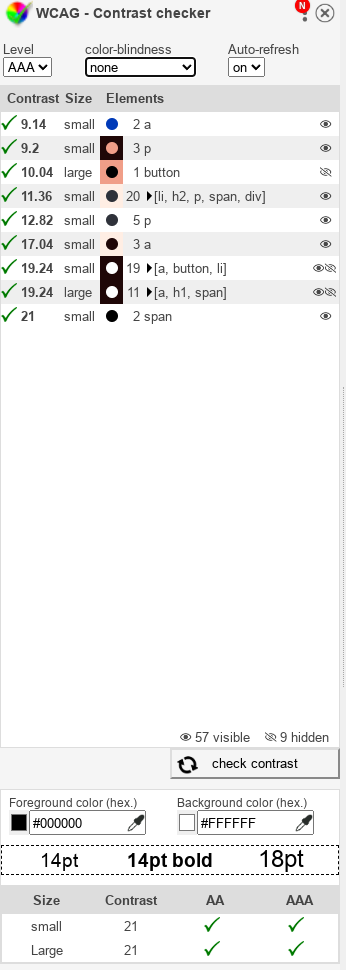
\includegraphics[scale=0.7]{src/contrasti/none.png}
		\caption{Contrasto dei colori in assenza di cecità cromatica.}
	\end{figure}
	\pagebreak
	\begin{figure}[H]
		\centering
		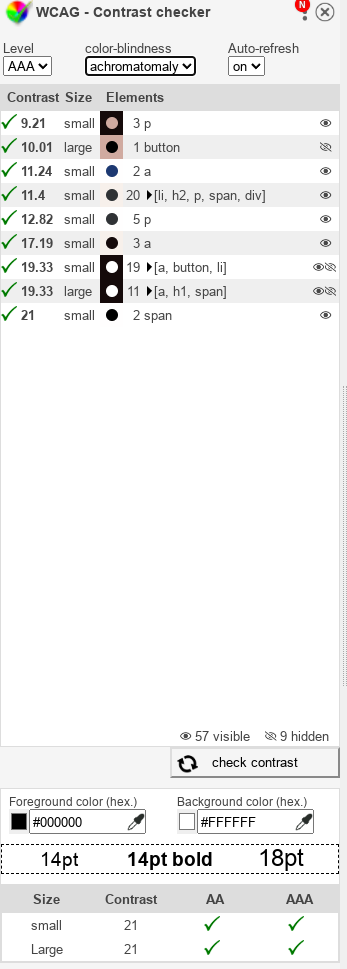
\includegraphics[scale=0.6]{src/contrasti/achromatomaly.png}
		\caption{Contrasto dei colori per gli affetti da acromatomalia.}
	\end{figure}
	\pagebreak
	\begin{figure}[H]
		\centering
		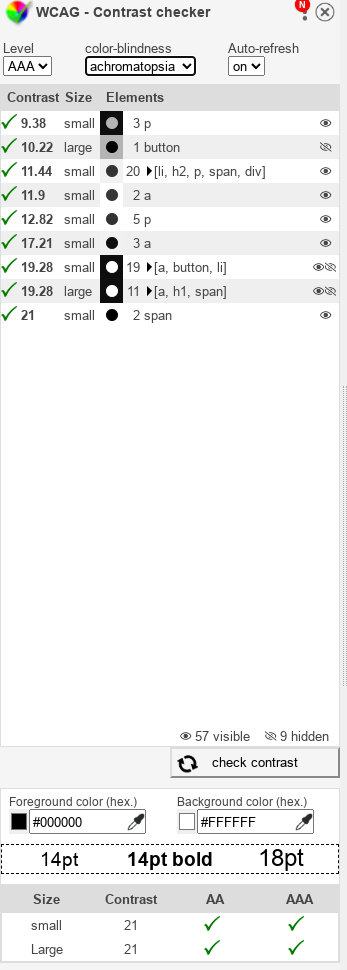
\includegraphics[scale=0.6]{src/contrasti/achromatopsia.png}
		\caption{Contrasto dei colori affetti da acromatopsia.}
	\end{figure}
	\pagebreak
	\begin{figure}[H]
		\centering
		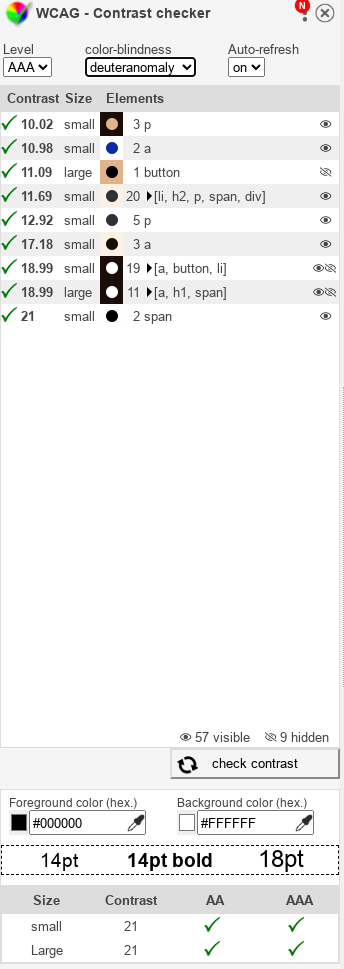
\includegraphics[scale=0.6]{src/contrasti/deuteranomaly.png}
		\caption{Contrasto dei colori per gli affetti da deuteronomalia.}
	\end{figure}
	\pagebreak
	\begin{figure}[H]
		\centering
		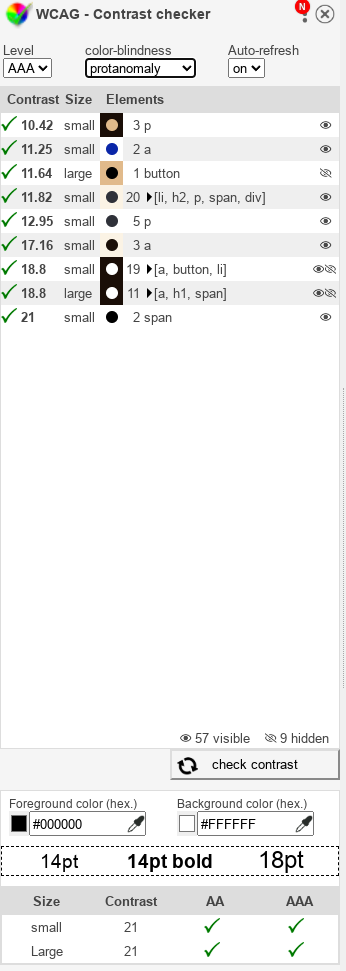
\includegraphics[scale=0.6]{src/contrasti/protanomaly.png}
		\caption{Contrasto dei colori per gli affetti da protanomalia.}
	\end{figure}
	\pagebreak
	\begin{figure}[H]
		\centering
		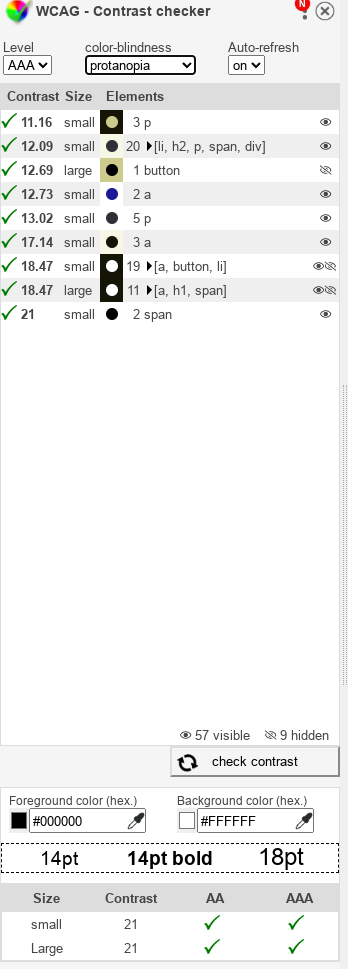
\includegraphics[scale=0.6]{src/contrasti/protanopia.png}
		\caption{Contrasto dei colori per gli affetti da protanopia.}
	\end{figure}
	\pagebreak
	\begin{figure}[H]
		\centering
		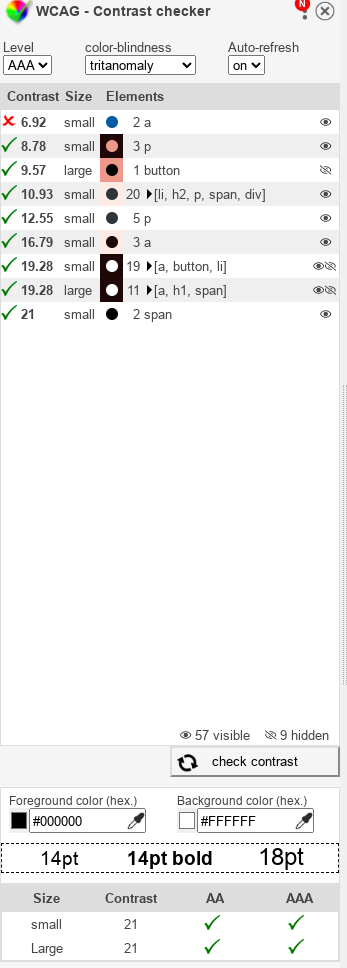
\includegraphics[scale=0.6]{src/contrasti/tritanomaly.png}
		\caption{Contrasto dei colori per gli affetti da tritanomalia.}
	\end{figure}
	\pagebreak
	\begin{figure}[H]
		\centering
		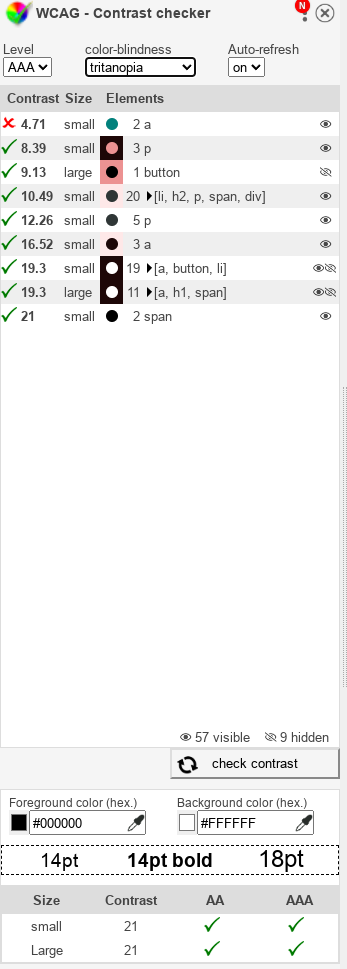
\includegraphics[scale=0.6]{src/contrasti/tritanopia.png}
		\caption{Contrasto dei colori per gli affetti da tritanopia.}
	\end{figure}
    \pagebreak
	\subsection{Noscript}
    L'elemento \textit{Noscript} è stato utilizzato per adattare elegantemente il sito a disposivi che non hanno \textit{Javascript} abilitato, in particolare è stato usato per:
    \begin{itemize}
        \item visualizzare una forma alternativa del menù a comparsa in formato \textit{mobile}.
        \item informare l'utente che la funzionalità del carrello locale è disattivata.
    \end{itemize}
	
	\subsection{Tabindex}
	L'utilizzo dell'attributo \textit{tabindex} è stato ridotto al minimo in quanto per la navigazione è naturalmente implementata dalla la corretta struttura delle pagine. \\
    l'unico punto in cui è stato utilizzato il \textit{tabindex} è stato per saltare al contenuto senza dover percorrere tutti \textit{link} presenti nell'\textit{header}. 

	\section{Presentazione}
	Per il sito è stato adottato un design fluido, con dei punti di rottura per i diversi dispositivi
	Per quanto riguarda la presentazione, tramite \textit{CSS} abbiamo implementato un design fluido e scalabile evitando il più possibile misure fisse, favorendo l'uso di misure relative alle preferenze dell'utente. Nella visualizzazione del menù è stato abbiamo utilizzato layout \textit{flex} e \textit{grid} che garantiscono una trasformazione elegante nella presentazione dei piatti, che seguisse un layout a griglia.

	\subsection{Desktop}
	\begin{figure}[H]
		\centering
		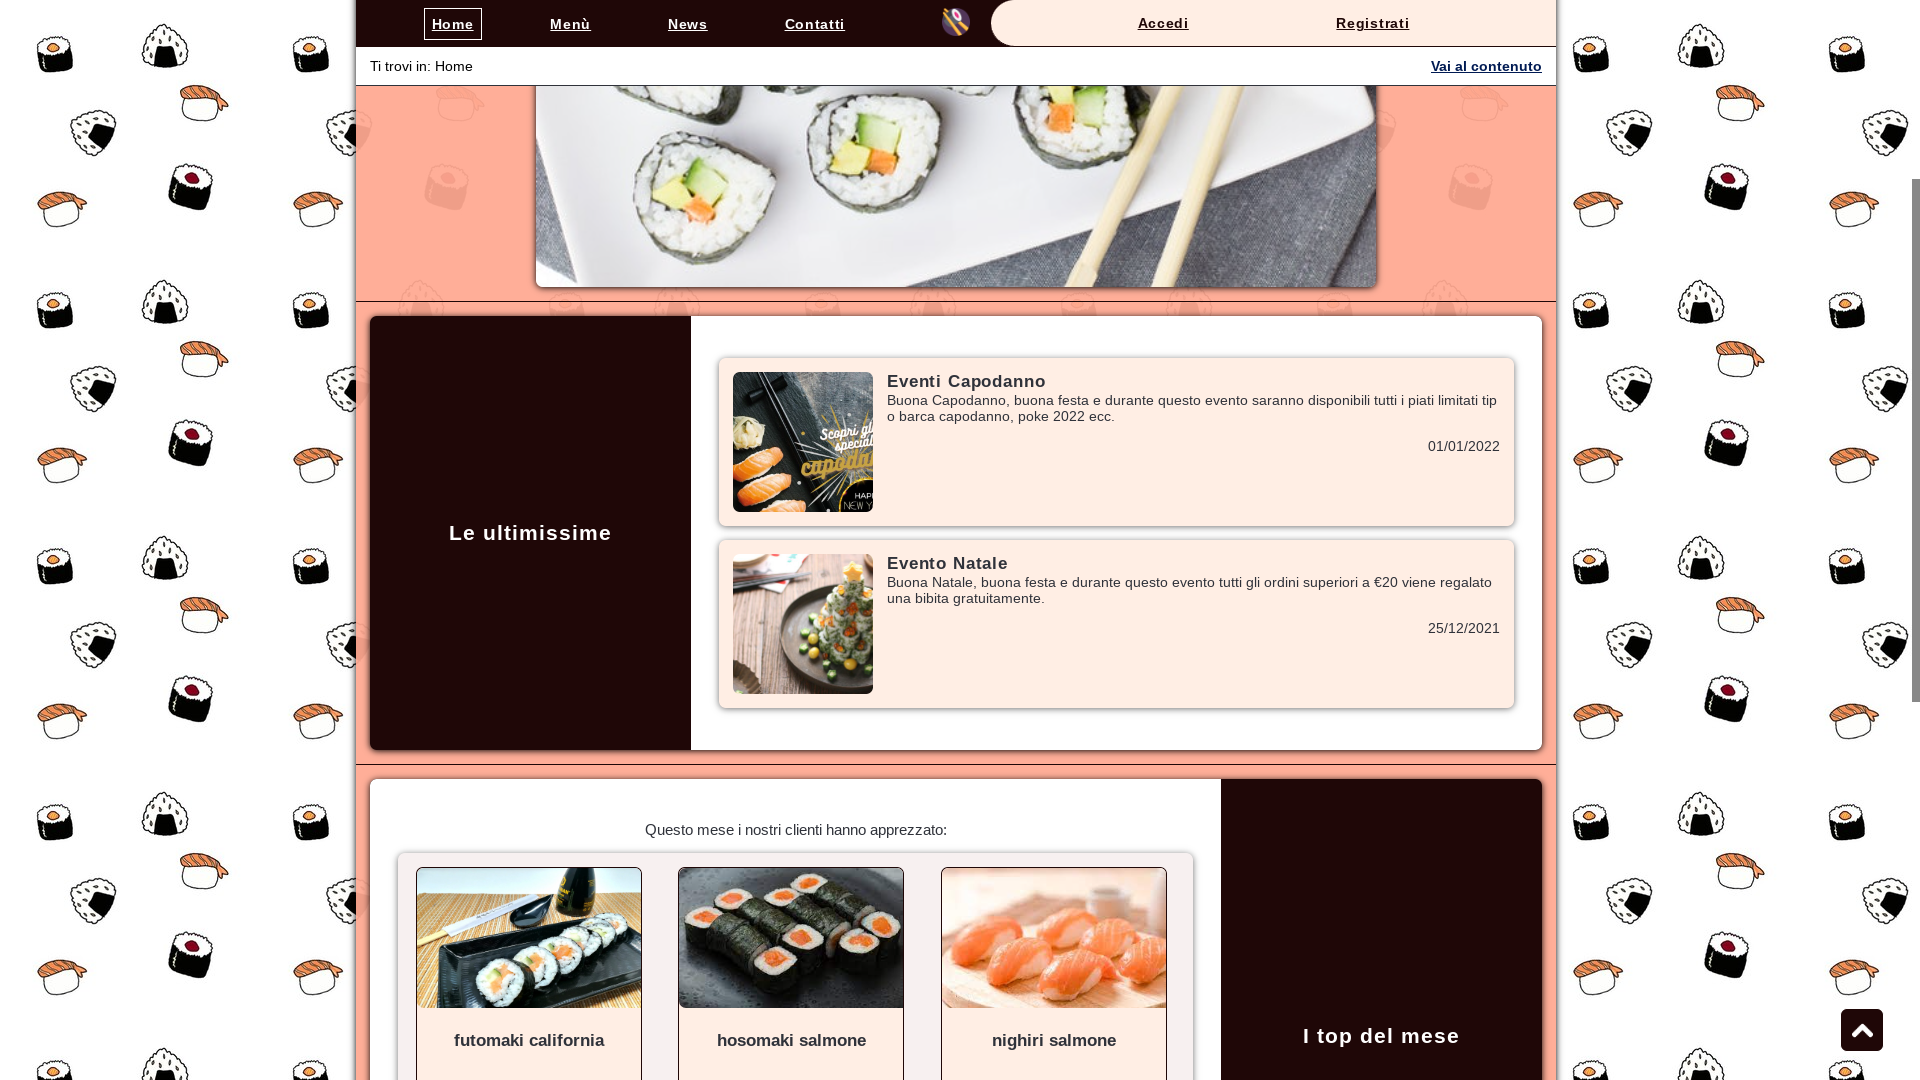
\includegraphics[scale=0.2]{src/layout/desktop.png}
		\caption{Layout desktop}
	\end{figure}

	\subsection{Tablet}
	\begin{figure}[H]
		\centering
		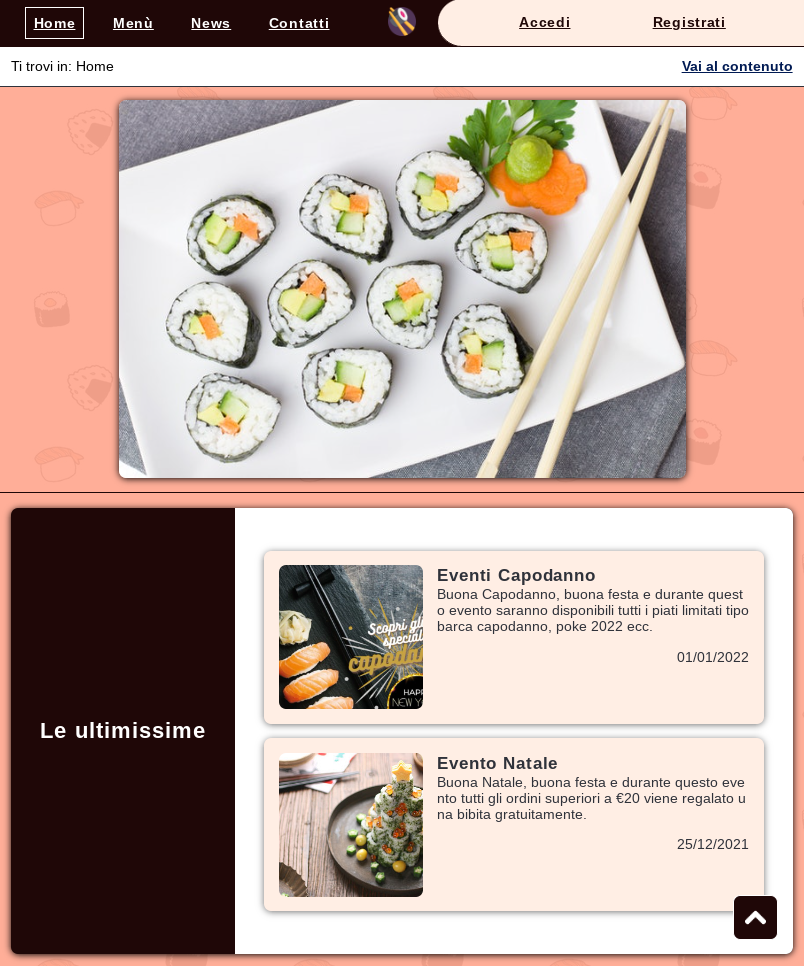
\includegraphics[scale=0.5]{src/layout/tablet.png}
		\caption{Layout tablet}
	\end{figure}

	\subsection{Mobile}
	\begin{figure}[H]
		\centering
		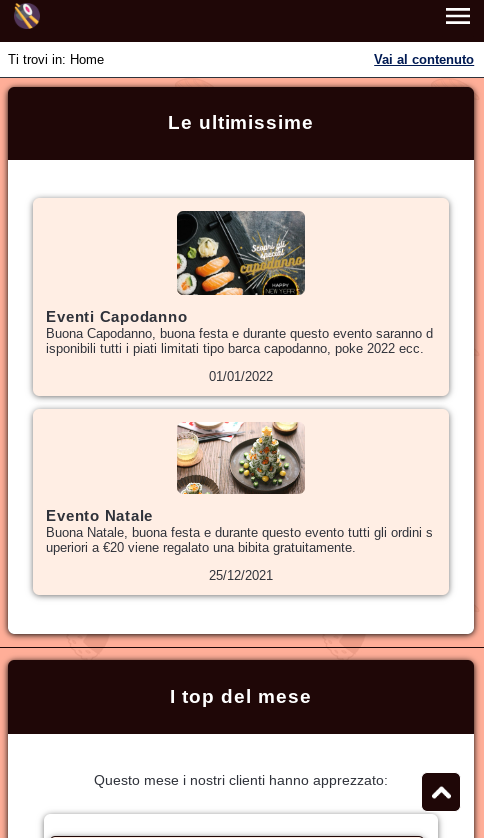
\includegraphics[scale=0.6]{src/layout/phone.png}
		\caption{Layout mobile}
	\end{figure}

	\subsection{Stampa}
	\begin{figure}[H]
		\centering
		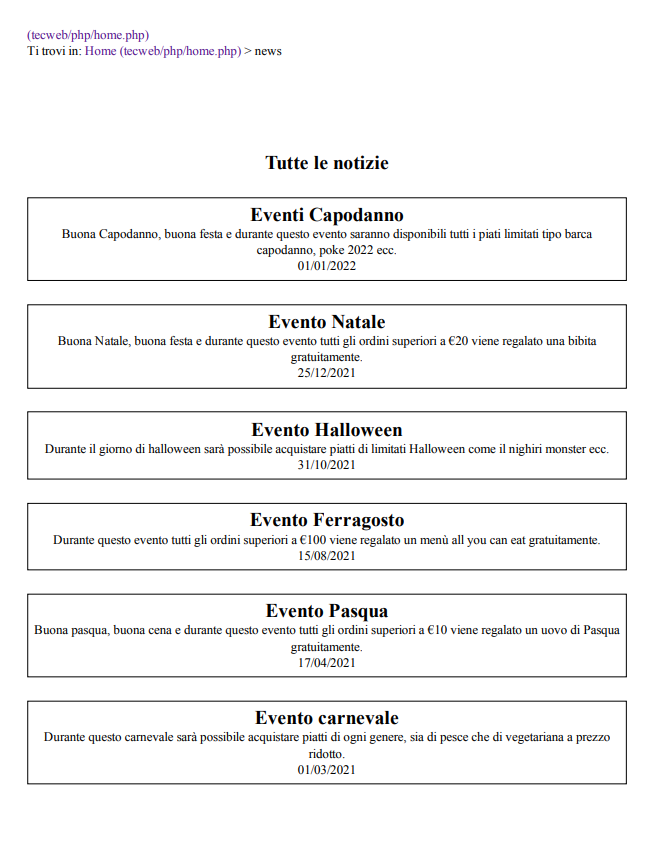
\includegraphics[scale=0.55]{src/layout/print.png}
		\caption{Layout di stampa}
	\end{figure}

	Il \textit{layout} di stampa mira a rimuovere gli elementi superflui (come footer, header, immagini di \textit{layout} e bottoni rilevanti) e mantenere solo il contenuto della pagina, lasciando comunque informazioni essenziali per comprendere il contesto della pagina, come il nome, breadcrumb e titolo della pagina e sezione.
	Il \textit{font} utilizzato nella stampa è il \textit{serif}, per questioni di leggibilitò, le immagini inoltre vengono ridotte al minimo indispensabile, mantenendolo solo per i piatti. Oltre a ciò il \textit{link} visualizzano il percorso di arrivo, il sito poi adatta il layout in modo da renderlo piacevole anche in \textit{layout} di stampa.

	\section{Comportamento}
	\subsection{Javascript}
	Per il comportamento di determinate pagine del sito, lato \textit{client}, è stato utilizzato un unico file \textit{Javascript} che comprende diverse funzioni, la maggior parte per far segnalare gli errori nell'\textit{input agli utenti}, in quanto il controllo di integrità dei dati è demandato alle funzionalità di \textit{HTML5}, per quanto riguarda i controlli lato \textit{client}, assegnando i giusti attributi ai \textit{tag <input>}. Proprio per questo motivo nei vari \textit{<input>} abbiamo utilizzato gli attributi required, pattern, maxlength, min e max. Inoltre, usando l'attributo title, quando è presente un errore nell'\textit{input} e viene inviato il form}, la pagina \textit{HTML} di \textit{default} fa visualizzare all'utente un messaggio di errore contenente la stringa dell'attributo title. Questo rende il codice Javascript relativo alla visualizzazione dei messaggi di errore una funzionalità aggiuntiva ma non essenziale. Siccome il solo controllo di integrità dei dati lato \textit{client} non è sufficiente, tutte le nostre pagine \textit{PHP} che ricevono dati in input ne controllano la validità lato \textit{server} e in caso di non conformità fanno visualizzare un errore. In generale abbiamo fatto in modo che le funzioni \textit{Javascript} non fossero essenziali per il completo funzionamento del sito e infatti le nostre pagine web sono completamente fruibili con tutte le loro funzionalità anche con Javascript disabilitato.

	\subsubsection{Funzionalità}
	\begin{itemize}
		\item \textbf{initializeValidationForm()}: inizializza i controlli se nella pagina è presente un determinato \textit{form};
		\item \textbf{loading*()}: funzioni che assegnano i controlli ai vari elementi dei \textit{form} delle pagine attraverso le funzioni \textbf{setOnBlurValidationRegex} e \textbf{setOnBlurConfirmPassword};
		\item \textbf{*Validation()}: funzioni usate per controllare se certi elementi dei \textit{form}, che non si possono validare solo con gli attributi HTML, siano stati inseriti correttamente altrimenti viene bloccato l'invio dei dati al server; 
		\item \textbf{readOnlyAddress()}: funzione utilizzata per impostare in sola lettura la via a cui consegnare l'ordine se viene scelta la modalità take away;
		\item \textbf{showError()}: mostra un messaggio d'errore sotto ad un campo del \textit{form};
		\item \textbf{resetErrorMessage()}: rimuove un messaggio d'errore sotto ad un campo del \textit{form};
		\item \textbf{validateByRegex()}: valida un campo del \textit{form} attraverso una espressione regolare e nel caso non venga rispettata viene visualizzato un messaggio d'errore tramite \textbf{showError};
		\item \textbf{validateDate()}: valida la data e l'ora scelta dall'utente per la consegna dell'ordine e nel caso non venga rispettata viene visualizzato un messaggio d'errore tramite \textbf{showError};
		\item \textbf{checkConfirmPassword()}: controlla se la password di conferma è uguale alla password inserita in precedenza, in caso negativo visualizza un messaggio d'errore tramite \textbf{showError};
		\item \textbf{confirmOrder()}: conclude l'ordine corrente verificando che i dati dell'ordine siano validi e, se lo sono, prima di inviarli al server rimuove tutti i piatti da \textit{local storage};
		\item \textbf{addCart(e)}: aggiunge il piatto selezionato al carrello, aggiungendolo nel \textit{local_storage};
		\item \textbf{removeCart(index)}: rimuove il piatto del indice \textit"index"} dal carrello, rimuovendolo dal \textit{local_storage};
		\item \textbf{showCart()}: mostra il carrello e il suo contenuto, creando una lista di piatti, le relative quantità e prezzi controllando il local_storage, nel caso non ci siano piatti nel carrello viene visualizzato un messaggio di carrello vuoto;
		\item \textbf{start(user)}: funzione che inizializza il carrello, controllando il \textit{local_storage} e i piatti nel carrello creati dal server, aggiorna il local_storage nel caso la lista di piatti sono diversi;
	\end{itemize}
	
	\subsection{PHP}
	I file \textit{PHP} gestiscono la logica di \textit{business} del sito e sono strutturati nel seguente modo:
	\begin{itemize}
		\item un file \textit{PHP} per ogni pagina del sito, che ne gestisce gestisce la logica;
		\item un file \textit{PHP} per interfacciarsi alla base di dati sottostante;
		\item un file \textit{PHP} per la validazione dei dati;
		\item un file \textit{PHP} globale contenente le funzioni o variabili necessarie a tutte le altre pagine \textit{PHP};
	\end{itemize}

    \subsubsection{Validazione}
	La validazione dei dati avviene in ambo le parti con dalle espressioni regolari, nel \textit{client} sia tramite gli attributi \textit{built-in HTML5} di validazione, sia in \textit{Javascript} il quale effettua anche una pulizia. \\
	Nel \textit{server} avviene un secondo controllo e pulizia dei dati inviati, ma anche un controllo logico, come ad esempio controllare che un utente esista già prima di crearne uno uguale. 
	
    \subsubsection{Sicurezza}
	\begin{itemize}
		\item ogni richiesta contenente dati sensibili, come quelle di autenticazione o acquisto, viene inoltrata con una \textit{HTTP POST};
		\item la pagina di registrazione non indica quale credenziale sia scorretta al fallimento dell'autenticazione;
		\item tutti i parametri inviati sono validati, controllati e ripuliti sia lato \textit{client} che lat \textit{server};
		\item ogni \textit{query} è eseguita con dei \textit{prepared statement} per evitare \textit{SQL injection}.
	\end{itemize}

    \subsubsection{Sessioni}
	Le variabili di sessione php utilizzate sono le seguenti:
	\begin{itemize}
		\item \$\_SESSION["logged"] = \textit{true} se l'utente è autenticato, textit{false} altrimenti;
		\item \$\_SESSION["admin"] = \textit{true} se l'utente è autenticato è un amministratore, textit{false} altrimenti;
		\item \$\_SESSION["info_msg"] = contiene un messaggio di notifica per l'utente;
		\item \$\_SESSION["redirect_link"] = contiene il \textit{link} in cui reindirizzare l'utente dopo aver visualizzato un messaggio di notifica;
		\item \$\_SESSION["active_cart"] = contiene l'identificativo del carrello corrente dell'utente autenticato;
		\item \$\_SESSION["username"] = contiene l'\textit{username} dell'utente autenticato;
		\item \$\_SESSION["first_name"] = contiene il nome dell'utente autenticato;
		\item \$\_SESSION["email"] = contiene il cognome dell'utente autenticato;
		\item \$\_SESSION["first_name"] = contiene l'\textit{email} dell'utente autenticato;
	\end{itemize}

	\subsubsection{Classe SushiDB}
    Questa classe si occupa della comunicazione tra la base di dati sottostante e lo strato superiore di presentazione delle pagine, essa va a semplificare l'interazione e separa in modo netto le due parti, mettendo a disposizione le sole \textit{query} necessarie per il sito. \\
    SushiDB implementa inoltre diverse funzionalità utili:
    \begin{itemize}
		\item prepared statements per evitare \textit{SQL injection};
		\item lettura dei parametri di accesso alla base di dati da un file di configuraione esterno, ciò rende SushiDB indipendente dalle credenziali usate;
		\item esecuzione delle \textit{query} in un unico punto, per evitare duplicazione di codice, ogni metodo di SushiDB infatti richiama lo stesso metodo per eseguire la \textit{query}.
	\end{itemize}

	\section{Testing}
	\subsection{Validazione}
	Tutte le pagine html e i file css sono stati sottoposti alla validazione tramite l'uso dei tool descritti nella sezione relativa alla realizzazione.
	
	\subsection{Peso}
	Il peso di ogni pagina del sito è stato calcolato tramite lo strumento descritto nella sezione relativa alla realizzazione. Tutte le pagine eccetto la galleria (3.4 MB) non superano 1 MB di peso, non è stato possibile alleggerire il peso della galleria senza perdita di qualità delle immagini.
	
	\subsection{Browser e dispositivi}

	Il sito è stato testato direttamente sui seguenti sistemi operativi:
	\begin{itemize}
		\item Windows 10;
		\item Windows 11;
		\item MacOS;
		\item Linux;
		\item Android 10;
		\item Android 11.
	\end{itemize}

	Il sito è stato testato direttamente sui seguenti browser e versioni successive:
	\begin{itemize}
		\item Chrome v97;
		\item Firefox v96;
		\item Safari v15.2;
		\item Lynx v2.8.9.
	\end{itemize}   

	\section{Organizzazione del gruppo}
	\subsection{Processo di sviluppo}
    L'idea nasce dalla passione comune per il \textit{sushi}, dopo aver fissato le funzionalità di base rispettando i requisiti imposti, siamo passati alla definizione della base di dati che regge il sito. \\
    Successivamente è iniziata la definizione delle pagine, suddividendo il lavoro come descritto nella sezione sottostante. Dopo aver impostato una struttura e \textit{layout} generale in del sito abbiamo creato il file \textit{SushiDB} per interfacciarci alla base di dati e iniziare l'implementazione delle funzionalità; contemporanemente a ciò, è maturato lo stile grafico del sito. \\
    Dopo aver completato le funzionalità è iniziata la fase di \textit{testing} per sistemare i possibili malfunzionamenti, fino ad arrivare al prodotto completo. \\
    Questo processo si è svolto con riunioni a cadenza settimanale, nelle quali si sono discussi gli avanzamenti e gli obiettivi a venire, ogni tre settimane inoltre è stato fatto un \textit{refactoring} del codice per facilitare la manutenibilità e lo sviluppo futuro. 
	
	\subsection{Divisione del lavoro}

	\subsubsection{Diego Stafa}
	\begin{itemize}
		\item definizione delle pagine, comprese dei relativi file \textit{HTML}, \textit{CSS}, \textit{JavaScript} e \textit{PHP} di: \textit{Home}, \textit{News}, \textit{News admin}, \textit{Contatti}, \textit{Info}, \textit{Modifica profilo}, \textit{Reimposta password};
		\item definizione dei file \textit{PHP}: \textit{SushiDB}, \textit{Errore 500}, \textit{validation.php};
		\item stile del sito.
	\end{itemize}

	\subsubsection{Luciano Wu}
	\begin{itemize}
		\item definizione delle pagine, comprese dei relativi file \textit{HTML}, \textit{CSS}, \textit{JavaScript} e \textit{PHP} di: \textit{Menù}, \textit{Menù admin};
        \item definizione della base di dati;
        \item popolazione della base di dati;
		\item controlli di accessibilità.
	\end{itemize}

	\subsubsection{Samuele Rizzato}
	\begin{itemize}
		\item definizione delle pagine, comprese dei relativi file \textit{HTML}, \textit{CSS}, \textit{JavaScript} e \textit{PHP} di: \textit{Carrello}, \textit{Area Personale}, \textit{Login}, \textit{Registrazione};
		\item definizione dei file \textit{PHP}: \textit{Global}, \textit{Logout}, \textit{Errore 404};
        \item validazione lato \textit{client}.
		\item definizione del file \textit{.htaccess}   
	\end{itemize}

\end{document}